\documentclass[12pt,a4paper]{article}

\usepackage[letterpaper]{geometry}

\usepackage{times}
\geometry{top=1.0in, bottom=1.5in, left=1.0in, right=1.0in}

\usepackage{fancyhdr}
\pagestyle{fancy}
\lhead{}
\rhead{}
\lfoot{}
\rfoot{}

\renewcommand{\headrulewidth}{0pt} 
\renewcommand{\footrulewidth}{0pt} 

\setlength\headsep{0.333in}

\usepackage{fontspec}
%\setmainfont{Times New Roman}

\usepackage{graphicx}

\usepackage{hyperref}

\usepackage{caption}

\usepackage{indentfirst}

\usepackage{setspace}

\usepackage{float}

\usepackage{enumitem}
\usepackage{listings}
\usepackage{color}
\usepackage{xcolor}

\usepackage{tabularx}

\usepackage{amsmath}

\begin{document}

\begin{titlepage}
\begin{center}
\vspace*{2cm}

\doublespacing
\rule{\linewidth}{0.3mm}

\textsc{
	\large
	UM-SJTU Joint Institute\\ 
	Physical Laboratory\\
	VP141
}

\rule{\linewidth}{0.3mm}


\vspace*{3.5cm}

{
\Large
\textsc{Laboratory Report}\\
}

\vspace*{0.2cm}

{
\large
\textsc{Exercise 1} \\
\textsc{Measurements of the Moment of Inertia}
}

\end{center}

\vfill
\normalsize

\hspace*{1cm}
\begin{minipage}{0.4\textwidth}
\begin{tabular}{p{1.7cm}p{4cm}llll}
Name: &  Ren Wang \hspace*{0.5cm} {\fontspec{Hei}\selectfont 王韧} & ID: & 516370910177 & Group: & 11 \\
\multicolumn{6}{l}{Date: \today}
\end{tabular}
\end{minipage}

\end{titlepage}

%\setmainfont{Times New Roman}
\onehalfspacing 
\newpage

\section{Introduction}
Fluid viscosity is one of the most important properties of fluids, determining
the fluid’s flow. 
Motion of an object in a fluid is hindered by a drag force acting in the
direction opposite to the direction of motion, i.e. opposite to the object’s
velocity. 

The magnitude of the drag force is related to the shape and speed of the object
as well as to the internal friction in the fluid.
The method used in this lab is known as Stokes’ method and it a common and
simple method for characterizing transparent or translucent fluids with high
viscosity.


% theoretical
Motion of an object in a fluid is hindered by a drag force acting in the
direction opposite to the direction of motion, i.e. opposite to the object’s
velocity. 
The magnitude of the drag force is related to the shape and speed of the object
as well as to the internal friction in the fluid.

This internal friction can be quantified by a number known as the viscosity
coefficient $\mu$.
For a spherical object with radius R moving at speed v in an infinite volume of
a liquid, the magnitude of the drag force is usually modeled as linear in the
speed
$$  F_1 = 6 \pi \mu v R  $$

When a spherical object falls vertically downwards in a fluid, it is being acted
upon by the following three forces:
The viscous force \emph{$F_1$} and the buoyancy force \emph{$F_2$} both act
upwards, and the weight of the object \emph{$F_3$} is directed downwards.
The magnitude of the buoyancy force is
$$  F_2 = \frac{4}{3} \pi R^3 \rho_1 g $$
where $\rho_1$ is the density of the fluid and $g$ is the acceleration due to
gravity. The weight of the object
$$  F_3 = \frac{4}{3} \pi R^3 \rho_2 g $$
with $\rho_2$ being the density of the object. After some time, the three forces
will balance each other
$$  F_1 + F_2 = F_3  $$
so that the net force on the object will be zero and from that instant on, the
object will be moving with constant speed $v_t$, known as the terminal speed.
Applying the condition, we can find
$$  \mu = \frac{2}{9} g R^2 \frac{\rho_2 - \rho_1 }{v_t}  $$
Therefore, the fluid viscosity can be found by measuring the terminal speed.
Taking into account that the motion with terminal speed is a motion with
constant velocity, the equation can be rewritten as
$$  \mu = \frac{2}{9} g R^2 \frac{( \rho_2 - \rho_1 ) t  }{s}  $$
where $s$ is the distance traveled in time $t$ after reaching the terminal
speed.

Since the volume of the fluid used in the measurement is not infinite, the
results are affected by some boundary effects due to the presence of the
container.

Therefore, the equation should be modified, and the formula for the
corrected magnitude of the viscous force for a infinitely long cylindrical
container with radius $R_c$ is 
$$  F_1 = 6 \pi \mu v R (1 + 2.4 \frac{R}{R_c})  $$
Consequently,
$$ \mu = \frac{2}{9} g R^2 \frac{( \rho_2 - \rho_1 ) t  }{s} (1 + 2.4
\frac{R}{R_c})  $$
Since the length $L$ of the container is limited, there may be further
corrections introduced, depending on the ratio on $\frac{R_c}{L}$. 







\newpage
\section{Experimental Setup}

The experimental setup consists of a Stokes’ viscosity measurement device (see
Figure 1) filled with castor oil in which motion of small metal balls will be
observed.

Measurements of various physical quantities in the experiment are performed with
a number of measurement devices: micrometer, calliper, densimeter, electronic
scales, stopwatch, and thermometer.

\begin{figure}[H]
\centering
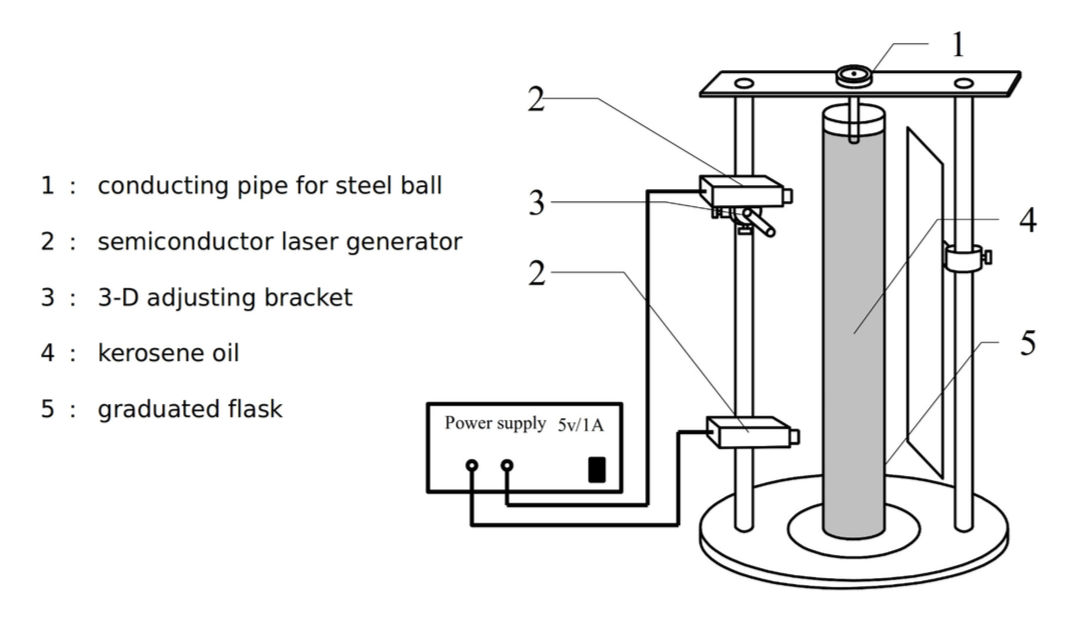
\includegraphics[width=12cm]{fig/p1}
\caption{Stokes viscosity measurement apparatus}
\end{figure}



\section{Measurement Procedue}

\setenumerate[2]{label=(\arabic*)}

\begin{enumerate}
\item Adjustment of the Stokes’ viscosity measurement device.

\begin{enumerate}
\item Adjust the knobs beneath the base to make the plumb aiming at the center
  of the base. 
\item Turn on the two lasers, adjust the beams so that they are parallel and aim
  at the plumb line. 
\item Remove the plumb and place the graduated flask with castor oil at the
  center of the base. 
\item Place the guiding pipe on the top of the viscosity measurement device.
\item Put a metal ball into the pipe and check whether the ball, falling down in
  the oil, can blocks the laser beams. If not, repeat Step 1.
\end{enumerate}

\item Measurement of the (constant) velocity of a falling ball.

\begin{enumerate}
\item Measure the vertical distance s between the two laser beams at least three
  times. 
\item Put a metal ball into the guiding pipe. Start the stopwatch when the ball 
  passes through the first beam, and stop it when it passes through the second
  one. Record the time $t$ and repeat the procedure for at least six times. 
\end{enumerate}

\item Measurement of the ball density $\rho_2$.

\begin{enumerate}
\item Use electronic scales to measure the mass of 40 metal balls. Calculate the
  average to find the mass of a single ball. 
\item Use a micrometer to measure the diameter of the metal balls. Repeat for
  ten times and calculate the average value. 
\item Calculate the ball density $\rho_2$.
\end{enumerate}

\item Measure of the density $\rho_1$ of the castor oil by using the provided
  densimeter (one measurement). Use a calliper to measure the inner diameter $D$
  of the graduated flask for six times. Read the ambient temperature from the
  thermometer placed in the lab. 
\item Calculate the value of viscosity coefficient $\mu$ using Eq. (5).

\end{enumerate}



\section{Caution}
\begin{itemize}
\item Do not move the graduated flask during the measurement.
\item Be careful with the castor oil: do not spill it on the desk.  
\item Do not forget to read the ambient temperature, as fluid viscosity is
  sensitive to the temperature. 
\end{itemize}



\section{Result}
\subsection{Distance Between Two Lasar Device}

\begin{table}[H]
  \centering
  \begin{tabular}{|l|c |c |c |}
    \hline
    \multicolumn{4}{|c|}{distance $S$ [mm] $\pm$ 1 [mm]} \\
    \hline
    S &  Ruler Start Point & Ruler End Point & Calculated Length \\
    \hline
    $S_1$ & 30.0 & 177.0 & 147.0 \\ \hline
    $S_2$ & 60.0 & 207.0 & 147.0 \\ \hline
    $S_3$ & 40.0 & 186.5 & 146.5 \\ \hline
  \end{tabular}
  \caption{Distance measurement data.}
\end{table}

Then we can find
$$  \bar{S} = \frac{1}{3} \sum_{k=1}^{3} S_k = 146.8 mm \pm 1 mm   $$
$$  u_{S,r} = 0.68 \%  $$ 


\subsection{Time Measurement}

\begin{table}[H]
  \centering
  \begin{tabular}{|l|c|}
    \hline
    \multicolumn{2}{|c|}{time $t$ [s] $\pm$ 0.01 [s] } \\
    \hline
    $t_1$ & 6.75 \\ \hline
    $t_2$ & 6.82 \\ \hline
    $t_3$ & 6.91 \\ \hline
    $t_4$ & 6.88 \\ \hline
    $t_5$ & 6.91 \\ \hline
    $t_6$ & 6.84 \\ \hline
  \end{tabular}
  \caption{Time measurement data.}
\end{table}


Then we can find
$$  \bar{t} = \frac{1}{6} \sum_{k=1}^{6} t_k =6.85 s \pm 0.01 s   $$
$$  u_{t,r} = 0.15 \%  $$ 

\subsection{The Diameters of The Balls}

The initial reading of the meter is 0.38 mm.
Thus, the raw data of measurement should firstly minus 0.38 mm, and is presented
as following, 

\begin{table}[H]
  \centering
  \begin{tabular}{|p{2cm}|p{3cm}||p{2cm} |p{3cm} |}
    \hline
    \multicolumn{4}{|c|}{diameter $d$ [mm] $\pm$ 0.005 [mm]  } \\
    \hline
    $d_1$ & 1.995 & $d_6$ & 1.995 \\ \hline
    $d_2$ & 1.995 & $d_7$ & 2.000 \\ \hline
    $d_3$ & 2.000 & $d_8$ & 1.800 \\ \hline
    $d_4$ & 1.995 & $d_9$ & 1.995 \\ \hline
    $d_5$ & 2.000 & $d_{10}$ & 1.995 \\ \hline
  \end{tabular}
  \caption{Ball diameter measurement data.}
\end{table}

Then we can find
$$  \bar{d} = \frac{1}{10} \sum_{k=1}^{10} d_k = 1.977  mm \pm  0.005 mm   $$
$$  u_{t,r} =  0.25 \%  $$ 

\subsection{The Inner Diameter of The Flask}

\begin{table}[H]
  \centering
  \begin{tabular}{|p{1cm}|c|}
    \hline
    \multicolumn{2}{|c|}{diameter $D$ [mm] $\pm$ 0.02 [mm]  } \\
    \hline
    $D_1$ & 61.40 \\ \hline
    $D_2$ & 61.46 \\ \hline
    $D_3$ & 61.20 \\ \hline
    $D_4$ & 61.36 \\ \hline
    $D_5$ & 61.20 \\ \hline
    $D_6$ & 61.50 \\ \hline
  \end{tabular}
  \caption{Flask diameter measurement data.}
\end{table}


Then we can find
$$  \bar{D} = \frac{1}{6} \sum_{k=1}^{6} D_k =  61.3533 mm \pm  0.02 mm   $$
$$  u_{D,r} =   0.03\%  $$ 


\subsection{Other Physical Quantities}

\begin{table}[H]
  \centering
  \begin{tabular}{|c|c|}
    \hline
    density of the castor oil $ \rho_1 [g/cm^3] \pm 0.001 [g/cm^3] $ & 0.955  \\ \hline 
    mass of 40 metal balls $ m  [g] \pm 0.001 [g] $ & 1.357 \\ \hline
    temperature in the lab $ T  [\circ C] \pm 2 [\circ C] $ & 25 \\ \hline
    acceleration due to gravity in the lab $ g [m/s^2] $ & 9.794 \\ \hline
  \end{tabular}
  \caption{Other Physical Quantities Measurement}
\end{table}

\subsection{Calculation of Density of One Ball}

The mass of one  metal ball can be calculated as
$$  m_0 = \frac{m}{40} = \frac{1.357 \times 10^{-3} }{40} = 3.3925 \times 10^-5 kg
\pm (2.500 \times 10^-8) kg $$ 
We can furtherly get the density,
$$ \rho_2 = \frac{m_0}{\frac{1}{6} \pi d^3} = \frac{3.3925 \times 10^-5
}{\frac{1}{6} \times 3.151593 \times (1.977 \times 10^-3)^3 } = 8.385 \times
10^3 kg/m^3 \pm (5.756 \times 10  ) kg/m^3  $$
$$  u_{\rho_2,r} =   0.6875\%  $$ 

\subsection{Calculation For The Viscosity Coefficient}
From the last equation in introduction part
\begin{multline*}
\mu = \frac{2}{9} g R^2 \frac{( \rho_2 - \rho_1 ) t  }{s} (1 + 2.4
\frac{R}{R_c})  =  \frac{2 \times (1.977 \times 10^-3 \times \frac{1}{2})^2
  (8.385\times 10^3 - 0.595 \times 10^3 ) \times 9.974 \times 6.85 }{9 \times
  146.8\times 10^-3 \times (1 + 2.4 \times \frac{1.977}{61.3533})} \\
 = 0.7307 Pa \times s \pm (6.8329 \times 10^-3 ) Pa \times s 
 \end{multline*}
$$  u_{\mu,r} =  0.93512 \%  $$ 



\section{Measurement Uncertainty Analysis}

\subsection{Uncertainty of The Distance Measurement}
We use formula to calculate type-A uncertainty
\begin{multline*}
 u_A = t_{0.95} \sqrt{\frac{1}{3(3-1)} \sum_{k=1}^3{(S_k-\bar{S})^2} } = \\
4.30 \cdot \sqrt{1/6\cdot ( (147.0-  146.83)^2 +  (147.0-  146.83)^2 + (146.5-
  146.83)^2 ) } =   0.7 mm
\end{multline*}
And type-B uncertainty is $u_B = $ = 1 mm. Thus,

$$   u_s = \sqrt{u_A^2+u_B^2} = \sqrt{0.7^2+1^2} = 1.2 mm  $$
$$   u_{S,r} = 1.2 / 146.8 = 0.82 \% $$ 

\subsection{Uncertainty of The Time Measurement}
We use formula to calculate type-A uncertainty
\begin{equation}
 u_A = t_{0.95} \sqrt{\frac{1}{6(6-1)} \sum_{k=1}^6{(t_k-\bar{t})^2} } = 1.05
 \cdot 0.0252 = 0.0492 s
\end{equation}
And type-B uncertainty is $u_B = $ = 0.01 s. Thus,
$$   u_t = \sqrt{u_A^2+u_B^2} = \sqrt{0.0492^2+0.01^2} =  0.0502 s $$
$$   u_{t,r} = 0.050 / 6.8517= 0.73 \% $$ 


\subsection{Uncertainty of The Ball Diameter}
We use formula to calculate type-A uncertainty
\begin{equation}
  u_A = t_{0.95} \sqrt{\frac{1}{10(10-1)} \sum_{k=1}^{10}{(d_k-\bar{d})^2} }
 = 0.715  \cdot   0.0197 = 0.0141 s
\end{equation}
And type-B uncertainty is $u_B = $ = 0.005 mm. Thus,
$$   u_d = \sqrt{u_A^2+u_B^2} = \sqrt{0.0141^2+0.005^2} = 0.0150 mm $$
$$   u_{d,r} = 0.0150 / 1.977 =  0.76 \% $$ 

\subsection{Uncertainty of The Inner Diameter of The Flask}
We use formula to calculate type-A uncertainty
\begin{equation}
  u_A = t_{0.95} \sqrt{\frac{1}{6(6-1)} \sum_{k=1}^{6}{(D_k-\bar{D})^2} }
 = 1.05  \cdot 0.0523 =  0.0549 mm 
\end{equation}
And type-B uncertainty is $u_B = $ = 0.02 mm. Thus,
$$   u_D = \sqrt{u_A^2+u_B^2} = \sqrt{0.0549^2+0.02^2} = 0.0584 mm $$
$$   u_{D,r} = 0.0584 /  61.3533 =  0.095 \% $$ 

\subsection{Uncertainty of The Mass of The Ball}
We have $u_m $ for 40 balls, thus
$$   u_{m_0} = u_m /40 = 0.0001 / 40 / 1000 = 2.5 \cdot 10^{-8} kg  $$

\subsection{Uncertainty of The Density of One Ball}
From
$$   \rho_2 = \frac{6m_0}{ \pi d^3 } $$
Then we can find that
$$ u_{\rho_2} = \sqrt{(\frac{\partial \rho_2}{\partial m_0})^2(u_{m_0})^2 +
  (\frac{\partial \rho_2}{\partial d})^2(u_d)^2 
} = 96.70  $$ 
$$   u_{\rho_2,r} = u_{\rho_2 } / \rho_2  =  96.70 / 8.385 \cdot 10^3 =   1.14 \% $$ 
The code is included as matlab/cal1.m 


\subsection{Uncertainty of The Viscosity Coefficient}


$$ \mu = \frac{2}{9} g R^2 \frac{( \rho_2 - \rho_1 ) t  }{s} (1 + 2.4
\frac{R}{R_c})  $$

Thus,
$$ u_{\mu} = \sqrt{(\frac{\partial \mu}{\partial d})^2(u_d)^2
  + (\frac{\partial \mu}{\partial s})^2(u_s)^2
  + (\frac{\partial \mu}{\partial t})^2(u_t)^2
  + (\frac{\partial \mu}{\partial \rho_1})^2(u_{\rho_1})^2
  + (\frac{\partial \mu}{\partial D})^2(u_D)^2 }  $$ 
$$ u_{\mu}  =  1.4264 \cdot 10^{-2}   $$
$$ u_{\mu,r} =\frac{u_\mu}{\mu}=  1.42 \cdot 10^{-2}  / 0.7307 =   1.94 \% $$

The code is included as matlab/cal2.m 



\section{Conclusion and Discussion}

In this lab, we use Stokes’ method to measure fluid viscosity.
The liquid been chosen to measure the viscosity is  the castor oil in this
experiment.

We measures Distance $S$, Time $t$, Diameter of the ball $d$, Inner diameter of
the flask $D$, Density of one ball $\rho_2$, then calculate the viscosity
coefficient not directly.

The relative uncertainty of each physical quantity is quite small, thus our
measurement is very precise and the result is acceptable.

The reason for the accuracy is the nice design of the experiment and carefulness
throughout the experiment.
There are many systematical and random errors leading to the main uncertainty,
but a lot of methods are used to reduce them.

% NOTE: bonus Q
We use 40 balls to calculate the average mass of the ball.
For each ball's mass is quite small and very hard to measure due to the
uncertainty of equipment. We choose 40 instead of 10 to maintain 4 significant
numbers.

% NOTE: bonus Q
Actually the temperature has influence on $\mu$.
The higher temperature is, the more likely the molecule will move, making the
viscosity lower. 

My experiment setup is closer two the air conditioner than other people, so my
result may be slightly affect by the temperature. 

% NOTE: theoretical 
From a engineering website

\url{http://www.engineeringtoolbox.com/absolute-viscosity-liquids-d_1259.html} 
We know that the theoretical value of the viscosity of caster oil is  $0.650
Pa/s$, but the experiment result is $0.7307Pa/s$.
$$ u_{\mu,r} = (0.7307 - 0.650)/ 0.650 \times 100\%  =  12.42 \%   $$ 
The reason is the AC mentioned before cooling down the temperature of my
experiment setup.
We can see here lower temperature results in higher viscosity.


% NOTE: concerns
Furthermore, there are more problems that may cause uncertainty and error in this lab.
\begin{enumerate}
\item The distance between two laser device may not be measured precisely for
  the thread is not strictly perpendicular to the level. 
\item When measuring the time, human's reponse may cause some delay between
  seeing the light fading and pressing down the button on the watch. 
\end{enumerate}

Some ways to improve this lab
\begin{enumerate}
\item Adjust the experimental setup carefully to the level.
\item Throw the ball in the center of the cylinder and in the same position
  every time.
\item Try hard to reduce response time.
\end{enumerate}

\section{Reference}
\begin{enumerate}
\item  The international system of units (SI) (PDF) (2008 ed.). United States Department of Commerce, NIST Special Publication 330. pp. 29 \& 57.
\item “Exercise 2-Lab Manual” Qin Tian, Feng Yaming, Mateusz Krzyzosiak,Department of Physics, Shanghai Jiaotong University.  
\end{enumerate}

\section{Data Sheet}

% data sheet

\end{document}